\documentclass[14pt]{article} % article
\usepackage[utf8]{inputenc}
\usepackage{listingsutf8}
%\usepackage[T2A]{fontenc}
\usepackage[english]{babel}
\usepackage{amssymb,amsmath,amsfonts,amsbsy}
%\usepackage{mathtext}
%\usepackage{indentfirst}
\usepackage{tabularx}
\usepackage{booktabs}
\usepackage{graphicx}
\usepackage[center]{caption}
\captionsetup{justification=raggedright,singlelinecheck=false}
\usepackage{subcaption}
\usepackage{cite}
\usepackage{enumerate}
\usepackage{enumitem}
%%\usepackage[braket]{qcircuit}
\usepackage{marvosym}
\usepackage{multicol}
\usepackage{comment}
\usepackage{authblk}
\usepackage{lipsum}
%\usepackage{hyperref}
\graphicspath{{figs/}}
%\DeclareGraphicsExtensions{.pdf,.png,.jpg}
%\bibliographystyle{utf8gost780u}
%\usepackage{apacite}
%\bibliographystyle{apacite}

% Print line number page wisely 
%\usepackage[pagewise]{lineno}
%\linenumbers

%\renewcommand\linenumberfont{\normalfont\bfseries\normal}
%\renewcommand\linenumberfont{\normal}

\title{\vspace{-2.5cm}\textbf{Exploring the Shared Low-Dimensional Subspace of EEG and EOG Signals in Sleep Stages}}

%\author[1]{Ilia Golub}
\author[]{Ilia Golub}

%\author[1]{Pratit Kandel}

%\author[1]{Prosperity Oguama}
\author[]{Xueqing Li}


%\affil[1]{Gonda Multidisciplinary Brain Research Center, Bar-Ilan University, Ramat Gan, Israel}
\affil[]{Gonda Multidisciplinary Brain Research Center, Bar-Ilan University, Ramat Gan, Israel}
%\affil[4]{Institute of Natural Sciences and Mathematics, Ural Federal University, Ekaterinburg, Russia}
%\affil[5]{Department of Cardiology, Clinical Sciences, Lund University, Lund, Sweden}
%\affil[6]{Arrhythmia Clinic, Skane University Hospital, Lund, Sweden}
%\affil[*]{Correspondence: golub.ilia.ilya@gmail.com}

\setcounter{Maxaffil}{0}
\renewcommand\Affilfont{\itshape\small}
\date{}

\usepackage[onehalfspacing]{setspace}

\usepackage{listings}
\renewcommand{\lstlistingname}{Listing}
\lstset{language=Python,
        numbers=left,
        basicstyle=\small\ttfamily,
        breaklines=true,
        showstringspaces=false,
        stepnumber=1,         
        numbersep=5pt,          
        showspaces=false,       
        showtabs=false,         
        %frame=single,          
        tabsize=4,              
        captionpos=b,           
        breakatwhitespace=false,
        escapeinside={\%*}{*)}, 
        texcl=true
        }

%\usepackage[left=1cm, right=1cm, top=1cm, bottom=1cm]{geometry} % 2.5 1 1 2.5
\usepackage[a4paper, margin=0.5in]{geometry}


\usepackage[
    colorlinks=true,
    linkcolor=blue,
    filecolor=magenta,      
    urlcolor=cyan,
    pdftitle={CW-2},
    pdfauthor={Golub I},
    bookmarks=true,
    linktoc=all,
	final]{hyperref}

\usepackage[nottoc]{tocbibind}

\makeatletter
\renewcommand{\@biblabel}[1]{#1.}
\makeatother

\sloppy

\righthyphenmin=2

\renewcommand{\theenumi}{\arabic{enumi}.}
\renewcommand{\labelenumi}{\arabic{enumi}.} 
\renewcommand{\theenumii}{\arabic{enumii}.} 
\renewcommand{\labelenumii}{\arabic{enumi}.\arabic{enumii}.}
\renewcommand{\theenumiii}{\arabic{enumiii}.} 
\renewcommand{\labelenumiii}{\arabic{enumi}.\arabic{enumii}.\arabic{enumiii}.} 


\DeclareMathOperator{\rot}{rot}		% Определяем операции rot
\DeclareMathOperator{\diverg}{div}	% div
\DeclareMathOperator{\grad}{grad}	% grad
\DeclareMathOperator{\arth}{Arth}    % arc tanh
\DeclareMathOperator{\Ai}{Ai}
\DeclareMathOperator{\Bi}{Bi}

\setcounter{tocdepth}{1}

\begin{document}

% Title
\maketitle

% Abstract
\section{Abstract}

%\textbf{Background}\\
EEG and EOG signals are fundamental components of sleep monitoring, yet their joint dynamics remain underexplored. While these modalities are often treated separately, recent evidence suggests overlapping signal content and potential interactions that reflect underlying neurophysiological coordination. Understanding how this coordination evolves across sleep stages may reveal new insights into brain-eye communication during sleep.
\textbf{Aim}: To quantify how strongly EEG and EOG signals couple across human sleep stages.

%\textbf{Methods}\\
Overnight PSG from 29 adults were segmented into Wake, N1, N2, N3 and REM. Canonical correlation analysis (CCA) extracted the first two shared dimensions ($\rho_1$, $\rho_2$) in static stage-wise blocks and in 30 s sliding windows.

%\textbf{Results}\\
Stage-wise $\rho_1$ and $\rho_2$ increased from Wake to N3, with REM and N1 showing intermediate coupling. Time-resolved analysis confirmed greater strength and stability in deeper stages, while coupling entropy was highest in Wake and REM.

%\textbf{Conclusion}\\
EEG and EOG share a state-dependent low-dimensional subspace that is strongest in N3, high in N2, moderate in N1 and REM, and minimal in Wake. These findings refine our understanding of brain-eye interactions and support stage-aware sensing and analysis in sleep research.

\section{Introduction}

Sleep stages unfolds through non-rapid eye movement (NREM) sleep, comprising stages N1 to N3, and rapid-eye-movement (REM) sleep, classically scored with polysomnography that monitors electroencephalographic (EEG) activity and electrooculographic (EOG) signals related to eye movements~\cite{liu2021}. Growing evidence shows these two channels are not independent: ocular potentials contaminate frontal EEG, while EOG electrodes sample cortical rhythms, and exploiting this overlap improves automatic detection of REM and drowsiness~\cite{xu2025, safieddine2012}. Such findings imply that brain and eye signals cohabit a low-dimensional "communication subspace" whose geometry may vary with different state. Yet the strength and dynamics of this coupling across all stages remain unquantified.

In this study, we seek to quantify this shared subspace across sleep stages by extracting the primary dimensions of joint EEG-EOG variance and systematically assessing how their correlation strength and stability vary as a function of sleep stages. We operationalize this coupling using canonical correlation analysis (CCA), allowing us to track not only average synchrony but also the variability and dimensional richness of shared activity across stages. Using the public Apnea Positive Pressure Long-term Efficacy Study (APPLES) overnight PSG dataset~\cite{mueller_nsrr}, we applied canonical correlation analysis (CCA) to EEG and EOG signals to extract dominant joint components and assess their coupling strength during wake, N1, N2, N3, and REM stages, testing the hypothesis that coupling peaks in REM and diminishes in deeper NREM sleep.
 
\section{Methods}

\subsection{Dataset}

Data for this study were drawn from 29 adult participants in the APPLES dataset. For each subject, we analyzed four bipolar EEG channels (C3-M2, C4-M1, O1-M2, O2-M1) alongside two EOG channels (LOC and ROC), with all recordings segmented according to the five sleep stages: Wake (W), N1, N2, N3 and REM (R).

\subsection{Preprocessing}

Preprocessing was carried out in MNE-Python by first loading the EEG and EOG channels from EDF recordings and then importing the corresponding sleep stage annotations. We converted annotation timestamps to seconds relative to each recording's start time to ensure precise alignment with the signal data and excluded or corrected any segments with alignment issues. Finally, we extracted continuous EEG and EOG epochs for each labeled stage (W, N1, N2, N3, REM) to serve as inputs for our canonical correlation analyses.

\subsection{Dimensionality Reduction and Method Selection}

We initially compared EEG and EOG subspaces using PCA and ICA followed by subspace angle computation, but both yielded near-zero or ill-defined angles, offering little physiological insight. 

\subsection{Static Canonical Correlation Analysis (CCA)}
Stage-wise CCA on full-length segments showed a depth effect: $\rho_1$ increased from $0.55 \pm 0.14$ (Wake) to $0.86 \pm 0.06$ (N3), and $\rho_2$ from $0.32 \pm 0.15$ to $0.61 \pm 0.09$. One-way ANOVAs confirmed significance ($\rho_1$: $F(4,140)=24.4$, $p<0.001$; $\rho_2$: $F(4,140)=16.7$, $p<0.001$), indicating stronger EEG--EOG synchrony in deeper NREM stages.

We also computed the proportion of EEG/EOG variance captured by each canonical variate. On average, the first component explained $52$--$57\%$ of EEG and $52$--$63\%$ of EOG variance. In N3, variance was more evenly split between components, whereas in REM and Wake the first component dominated, indicating a compact but stage-dependent coupling structure.

\subsection{Time-Resolved CCA Analysis}
To track the temporal evolution of EEG--EOG coupling, the two-component CCA was applied in sliding windows of $30\,\mathrm{s}$ with a $15\,\mathrm{s}$ step ($50\%$ overlap). Values were then averaged into non-overlapping $10\,\mathrm{min}$ bins to visualise stage-specific trends with reduced high-frequency variability.

We analysed the results via: (i) \emph{stage-wise aggregation}---mean and dispersion of $\rho_1,\rho_2$ within each stage; (ii) \emph{overnight trajectories}---$10\,\mathrm{min}$ bin averages across the night; and (iii) \emph{distributional complexity}---per subject and stage, Shannon entropy, skewness, and kurtosis of the $\rho_1/\rho_2$ distributions.

Local stationarity of each $30\,\mathrm{s}$ window was tested with the Augmented Dickey--Fuller (ADF) and KPSS methods. Across $266$ segments, $85\%$ passed ADF and $61\%$ passed KPSS, with $56\%$ agreement; only $10.5\%$ failed both. Occasional KPSS statistics beyond tabulated $p$-value bounds were retained for consistency.

Stage differences were assessed with one-way ANOVA (\texttt{SciPy.stats}).

\section{Results}

\subsection{Static Canonical Correlation Analysis (CCA)}

Stage-wise CCA on full-length segments showed a clear depth effect. The first canonical correlation ($\rho_1$) rose from 0.55 $\pm$ 0.14 in Wake to 0.86 $\pm$ 0.06 in N3; the second ($\rho_2$) increased from 0.32 $\pm$ 0.15 to 0.61 $\pm$ 0.09 (\ref{fig:figure1}). One-way ANOVAs confirmed significance ($\rho_1$: F(4, 140)=24.4, p<0.001; $\rho_2$: F(4, 140)=16.7, p<0.001), indicating stronger EEG-EOG synchrony in deeper NREM sleep.

\begin{figure}
\centering
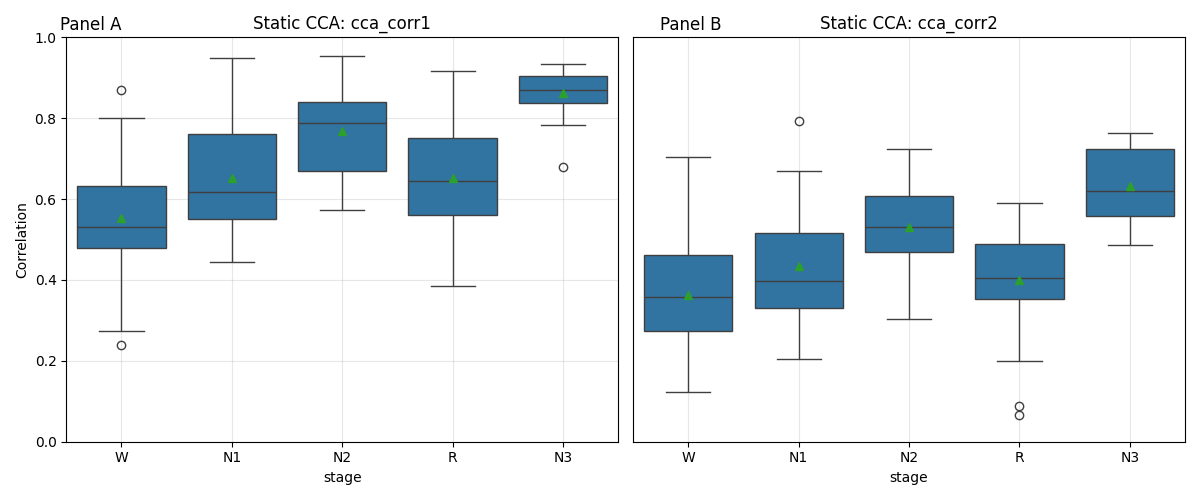
\includegraphics[width=0.8\textwidth]{figure1_static_cca_boxplots.png} % static_cca_analysis/cca_corr_by_stage.png
\caption{Static canonical correlation analysis (CCA) across sleep stages. Panel A shows the first canonical correlation ($\rho_1$), and Panel B shows the second ($\rho_2$), both increasing from Wake to N3.}\label{fig:figure1}
\end{figure}

\subsection{Time-Resolved CCA Analysis}

Sliding windows (30 s, $50\%$ overlap) reproduced the pattern with finer resolution. Aggregated $\rho_1$ ranged from 0.73 $\pm$ 0.13 (Wake) to 0.87 ± 0.07 (N3); $\rho_2$ from 0.45 $\pm$ 0.17 to 0.65 $\pm$ 0.11 (\ref{fig:figure2}). Variability diminished with depth, and 10-min bins revealed stable plateaus in N2/N3 but fluctuating profiles in REM and Wake. Transition phases (e.g., N1) showed inconsistent coupling patterns.

Local stationarity analysis confirmed that the majority of 30-second windows met standard weak stationarity criteria. Specifically, 85\% of the time-resolved segments passed the ADF test and 61\% passed the KPSS test, with both tests agreeing on stationarity in 56\% of cases. Only 10.5\% of windows were classified as non-stationary by both tests. These results justify the use of fixed-length sliding windows for estimating coupling dynamics.
\begin{figure}
\centering
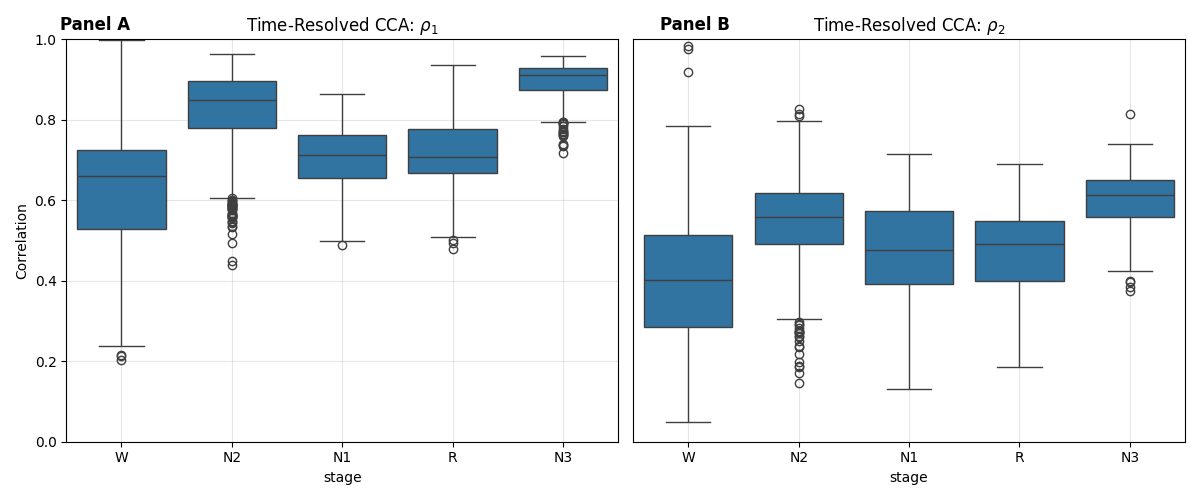
\includegraphics[width=0.8\textwidth]{figure2_time_resolved_boxplots.png} % static_cca_analysis/cca_corr_by_stage.png
\caption{Time-resolved CCA reveals stronger and more stable EEG-EOG coupling in deeper sleep stages.}\label{fig:figure2}
\end{figure}

\subsection{Distributional Complexity of Coupling Dynamics}

Entropy was highest in Wake and REM and lowest in N3 (\ref{fig:figure3}). Skewness (between -0.5 and 0.5) remained near zero, but kurtosis was elevated in Wake/REM, suggesting occasional extreme coupling events.

\begin{figure}
\centering
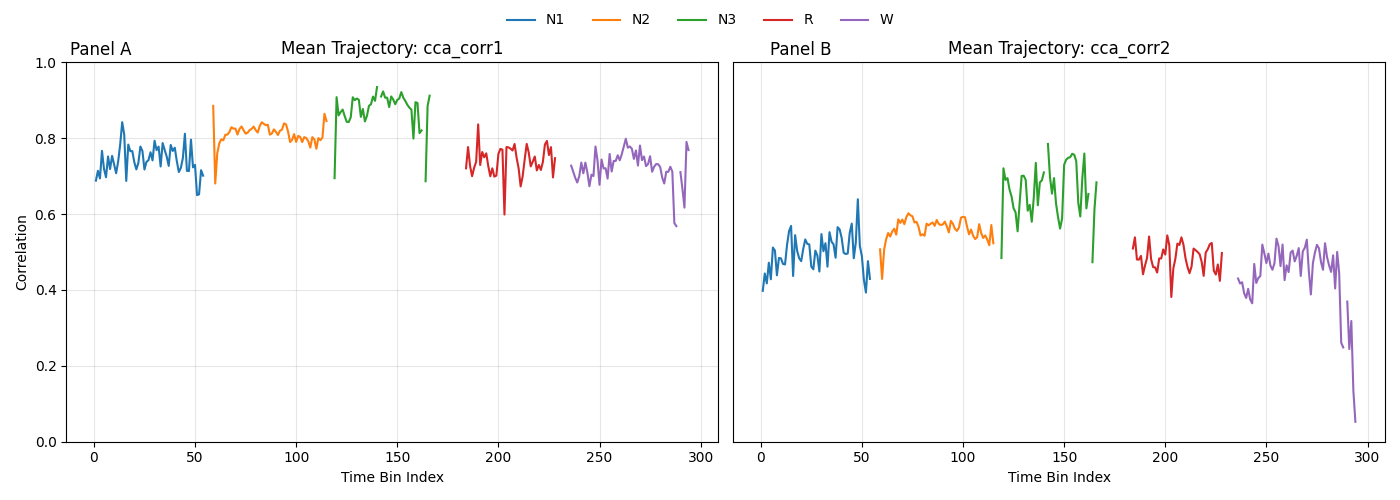
\includegraphics[width=0.8\textwidth]{figure3_cca_trajectories.png} % static_cca_analysis/cca_corr_by_stage.png
\caption{Coupling entropy is highest in Wake and REM, and lowest in N3.}\label{fig:figure3}
\end{figure}

\subsection{Projection Statistics and Downsampled Components}

Mean and variance of the individual canonical projections showed no stage effect (all ANOVA p > 0.17; \ref{fig:figure4}). Thus, stage differences stem from correlation structure rather than projection amplitude.

We also evaluated how much signal variance was captured by each canonical variate. On average, the first component explained 52-57\% of EEG variance and 52-63\% of EOG variance across sleep stages. In deeper stages such as N3, variance was more evenly distributed across components, while in REM and Wake, the first component dominated. These findings indicate a low-dimensional, structured coupling that varies with brain state.
\begin{figure}
\centering
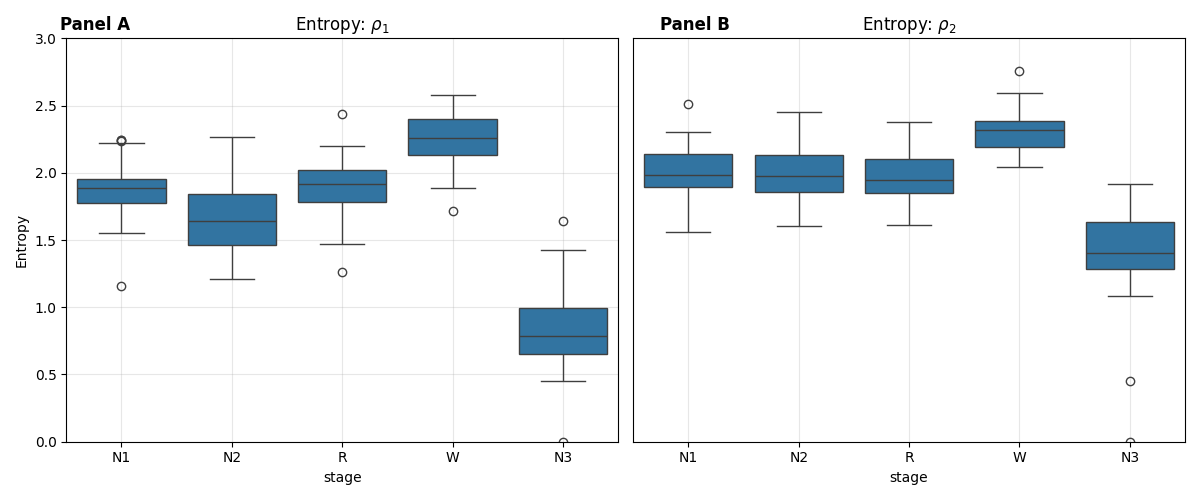
\includegraphics[width=0.8\textwidth]{figure4_entropy_boxplots.png}
\caption{Mean canonical projections remain stable across stages.}\label{fig:figure4}
\end{figure}

\section{Discussion}

This study quantified the low-dimensional communication subspace shared between EEG and EOG signals across sleep stages using CCA. Both static and time-resolved analyses revealed a robust increase in coupling strength with sleep depth: the first canonical correlation $\rho_1$ rose from 0.55$\pm$0.14 in Wake to 0.86$\pm$0.06 in N3, and the second $\rho_2$ from 0.36$\pm$0.15 to 0.63$\pm$0.10. REM and N1 showed intermediate coupling, closer to Wake than to N2/N3 --- a pattern replicated across time windows, further supporting the sleep-stage specificity of EEG-EOG coupling.
Temporal trajectories showed stable coupling in N2/N3 and greater variability in Wake and REM as they showing lower correlation values and higher entropy, supported by entropy measures. Lower entropy in deep sleep suggests more consistent EEG-EOG coordination, potentially reflecting reduced sensory input and motor variability. In contrast, higher entropy in Wake and REM may reflect more complex and dynamic brain-eye interactions. The persistent contribution of $\rho_2$ across all stages, especially in Wake and REM, suggests that EEG-EOG interactions are not dominated by a single mode, but instead reflect multiplexed coupling mechanisms in more active states. These findings may have practical implications for both research and clinical applications. Given the sensitivity of EEG-EOG coupling to sleep depth and stage transitions, CCA-derived features could enhance automatic sleep staging algorithms, particularly in distinguishing REM from N1 or Wake. Furthermore, altered coupling profiles may serve as markers of disrupted sleep architecture in conditions such as obstructive sleep apnea or REM behavior disorder. Future studies should investigate how these coupling metrics vary in pathological sleep and whether they offer diagnostic or prognostic value.
The analysis of explained variance provided additional insight into the geometry of the EEG-EOG subspace. The fact that just two canonical components captured nearly all relevant variance supports the hypothesis that EEG and EOG signals cohabit a compact, low-dimensional space. This compactness was most pronounced in N2 and N3, where variance was more evenly distributed across components, and less so in REM and Wake, which were dominated by a single component. These patterns mirror the stage-specific entropy and correlation results, reinforcing the interpretation that sleep depth modulates not only coupling strength, but also its complexity and dimensional shape.
Furthermore, our validation of local stationarity across the majority of analysis windows supports the reliability of time-resolved CCA estimates. The rare non-stationary windows—primarily in Wake and REM—likely reflect physiological transients or stage transitions rather than methodological artifacts. Together, these results strengthen the foundation for using CCA-based coupling metrics in sleep research.

\textbf{Limitations}
This study has several limitations. First, although preprocessing was applied, residual artifacts (e.g., blinks, muscle activity) may have influenced coupling estimates, especially in wake and REM stages. Second, the APPLES dataset includes individuals with varying sleep pathologies (e.g., OSAS), but we did not stratify by clinical status due to metadata constraints, limiting generalizability. Third, our analysis focused on a subset of EEG (C3, C4) and EOG (LOC, ROC) channels; while representative, this may miss spatially distributed coupling patterns. Fourth, our use of 10-minute time bins improved stability but may have smoothed out transient events during REM or stage transitions. Finally, CCA captures only linear relationships; incorporating nonlinear approaches (e.g., kernel CCA or mutual information) may reveal richer coupling dynamics in future work.

%\section{Conclusion}
\textbf{Conclusion}
This study shows that EEG and EOG signals share a low-dimensional subspace whose strength and temporal stability vary systematically across sleep stages. Coupling was strongest and most consistent in N3 and N2, moderate in N1 and REM, and weakest in Wake. These findings suggest structured coordination between cortical and oculomotor systems that tracks sleep depth. By focusing on intermodality dynamics via CCA, our approach offers a compact, interpretable view of sleep architecture that may inform future studies of sleep disorders and altered states.

\renewcommand{\baselinestretch}{1.5}
%\singlespacing
%\renewcommand\bibname{Bibliography}
\bibliographystyle{abbrv} %abbrv
\phantomsection     % 
\cleardoublepage    % 
\bibliography{report}

\end{document}
